%!TeX spellcheck = en-GB

\documentclass[hyperref={colorlinks=true,urlcolor=blue,linkcolor=.},aspectratio=1610,mathserif]{beamer}
\usepackage[utf8]{inputenc}
\usepackage{mathdots}
\usepackage{graphicx}
\usepackage[autoplay,loop,keepaspectratio]{animate}
\usepackage{minted}
\setminted{fontsize=\tiny}
\usemintedstyle{monokai}

\beamertemplatenavigationsymbolsempty
\usefonttheme{structuresmallcapsserif}
\usecolortheme{beaver}

\setbeamertemplate{footline}
{%
\begin{beamercolorbox}{section in foot}
\begin{center}
  \vskip2pt\insertnavigation{\paperwidth}\vskip2pt
\end{center}
\end{beamercolorbox}%
}

\setbeamersize{text margin left=30mm,text margin right=30mm}

\definecolor{DTUred}{cmyk}{0,0.91,0.72,0.23}
\definecolor{itemcolor}{cmyk}{0,0,0,0.56}
\definecolor{blockbodycolor}{cmyk}{0,1,1,0.5}
\definecolor{White}{cmyk}{0,0,0,0}
\setbeamercolor{titlelike}{fg=DTUred}
\setbeamercolor{section in head/foot}{fg=DTUred}
\setbeamercolor{section in toc}{fg=DTUred}
\setbeamercolor{itemize item}{fg=itemcolor}
\setbeamercolor{redbox}{fg=White,bg=blockbodycolor}

\title{Nanomechanics of Graphene Membranes}
\subtitle{vibrational modes on the nanoscale}
\author{\centering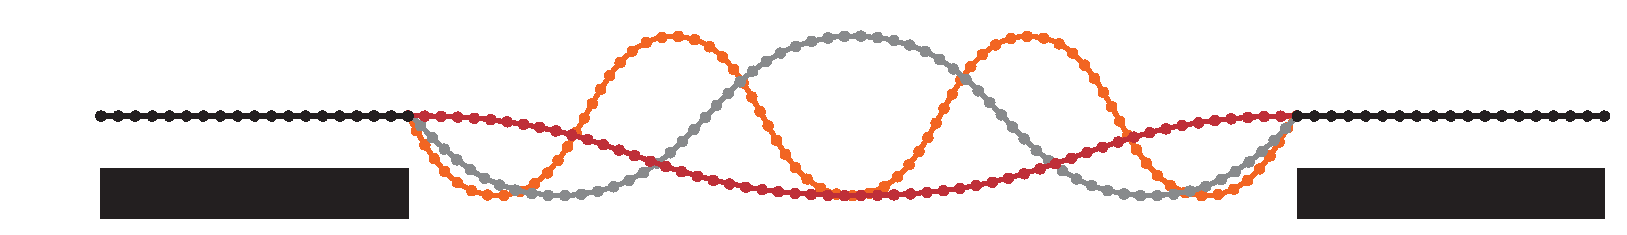
\includegraphics[width=8cm]{Miscellaneous/Graphics/Logo.eps}\\Christoffer Vendelbo Sørensen \and Frederik Grunnet Kristensen \and Rasmus Kronborg Finnemann Wiuff\\Supervisors: Mads Brandbyge \and Tue Gunst}
\institute{Technical University of Denmark}
\date{\today}

\begin{document}

\begin{frame}[plain]
 \titlepage
\end{frame}

\begin{frame}[plain]
 \frametitle{Outline}
 \tableofcontents
\end{frame}

\section{Introduction}

\begin{frame}
 \frametitle{Introduction}
 \begin{columns}[T]
  \column{0.7\textwidth}
  \begin{itemize}
   \item<1-> Graphene: 2D Carbon lattice
   \item<2-> Prominent properties
   \item<3-> Dejan Davidovikj, Jesse J. Slim, Santiago J. Cartamil-Bueno, Herre S J Van Der Zant, Peter G. Steeneken, and Warner J. Venstra\\
         “Visualizing the Motion of Graphene Nanodrums”\\
         \href{http://dx.doi.org/10.1021/acs.nanolett.6b00477}{Nano Letters \textbf{16}, 2768-2773 (2016)} \href{http://arxiv.org/abs/1602.00135}{arXiv:1602.00135}
   \item<4-> Microdrums on the micron scale
   \item<5-> Nanomembranes on the nanometer scale
  \end{itemize}
  \column{0.5\textwidth}<3->
  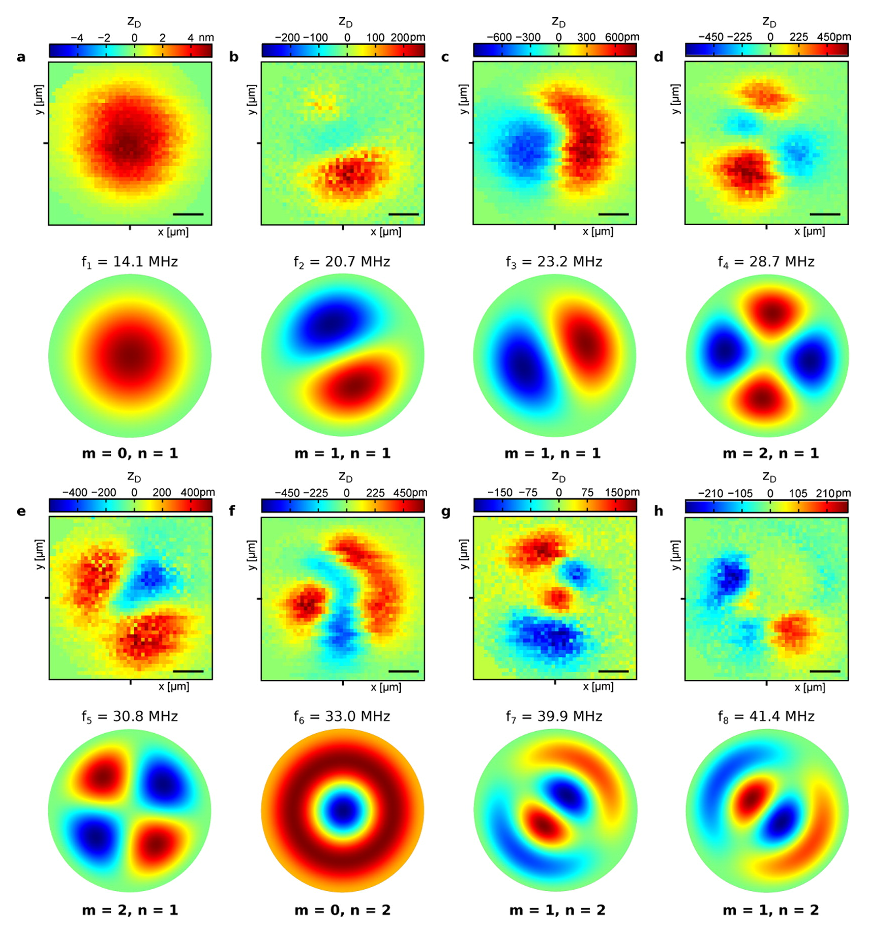
\includegraphics[width=\columnwidth]{Figures/motivation.eps}
 \end{columns}
\end{frame}

\begin{frame}
 \frametitle{Introduction}
 \begin{columns}[c]
  \column{0.4\textwidth}
  \begin{flushright}
      Hypothesis:
  \end{flushright}
  \column{\textwidth}
  \vskip1em
  \begin{beamercolorbox}[sep=1em,wd=8cm]{redbox}
      Does drum modes exist in graphene supported by a nanomesh with nanometersized holes?
  \end{beamercolorbox}
 \end{columns}
\end{frame}

\section{The Dynamical Matrix}

\begin{frame}
 \frametitle{The Dynamical Matrix}
 \begin{itemize}[<+->]
  \pause
  \item Matrix in Eigenvalue problem (below)
  \item Elements in matrix are Fouriertransform of the spring constants between configuration atoms
  \item Essential for calculating vibrational modes
 \end{itemize}
 \begin{equation}
  M\omega_{\mathbf{q}}^{2}
  \begin{bmatrix}
   A_{1} \\
   A_{2} \\
   A_{3}
  \end{bmatrix}
  =
  \begin{bmatrix}
   D_{11} & D_{12} & D_{13} \\
   D_{21} & D_{22} & D_{23} \\
   D_{31} & D_{32} & D_{33}
  \end{bmatrix}\begin{bmatrix}
   A_{1} \\
   A_{2} \\
   A_{3}
  \end{bmatrix} \nonumber
 \end{equation}
\end{frame}

\section{Our methods}

\subsection{ATKPython \& Simulating Nanomembranes}

\begin{frame}
 \frametitle{ATKPython \& Simulating Nanomembranes}
 \begin{columns}[T]
  \column{0.7\textwidth}
  \begin{itemize}
   \item<1-> Atomistic calculations
   \item<2-> HPC server cluster
   \item<3-> Workflow
         \begin{enumerate}
          \item<3-> Create Configuration
          \item<4-> Set potentials and optimise geometry
                \begin{itemize}
                 \item Intralayer: Tersoff-Brenner (2010)
                 \item Interlayer: Lennard-Jones:\begin{equation}
                        V_{ij}(r) = 4 \epsilon_{ij} \left[ \left( \frac{\sigma_{ij}}{r} \right) ^{12} - \left( \frac{\sigma_{ij}}{r} \right) ^6 \right] \nonumber
                       \end{equation}
                \end{itemize}
          \item<5-> Calculate the Dynamical Matrix
          \item<6-> Calculate the vibrational modes
         \end{enumerate}
   \item<7-> Analysing modes
  \end{itemize}
  \column{0.68\textwidth}<1->
  \begin{figure}
   \centering
   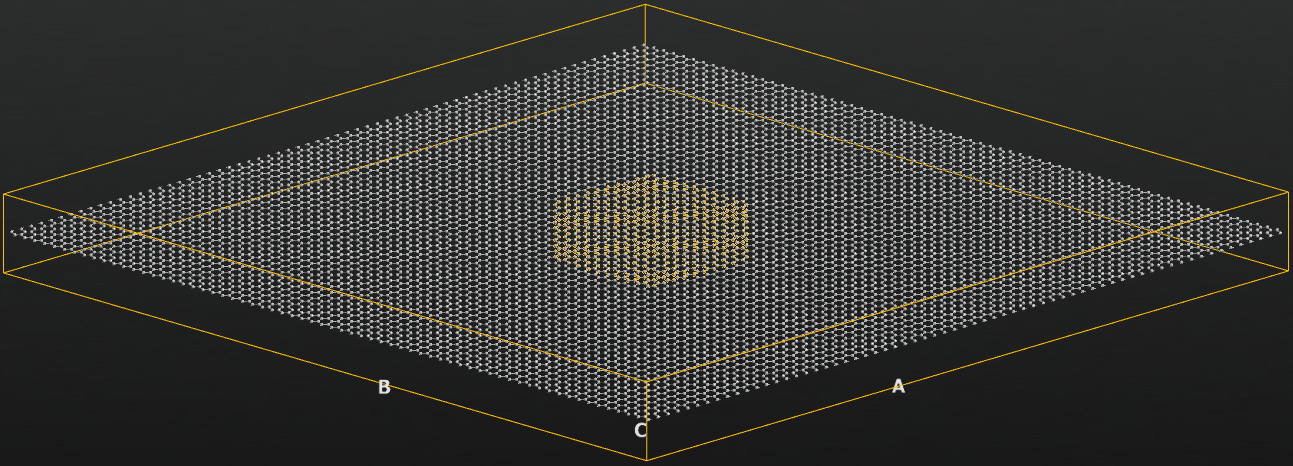
\includegraphics[width=\columnwidth]{Figures/NanoLayer5nm.png}
   \vspace{1em}
   \centering
   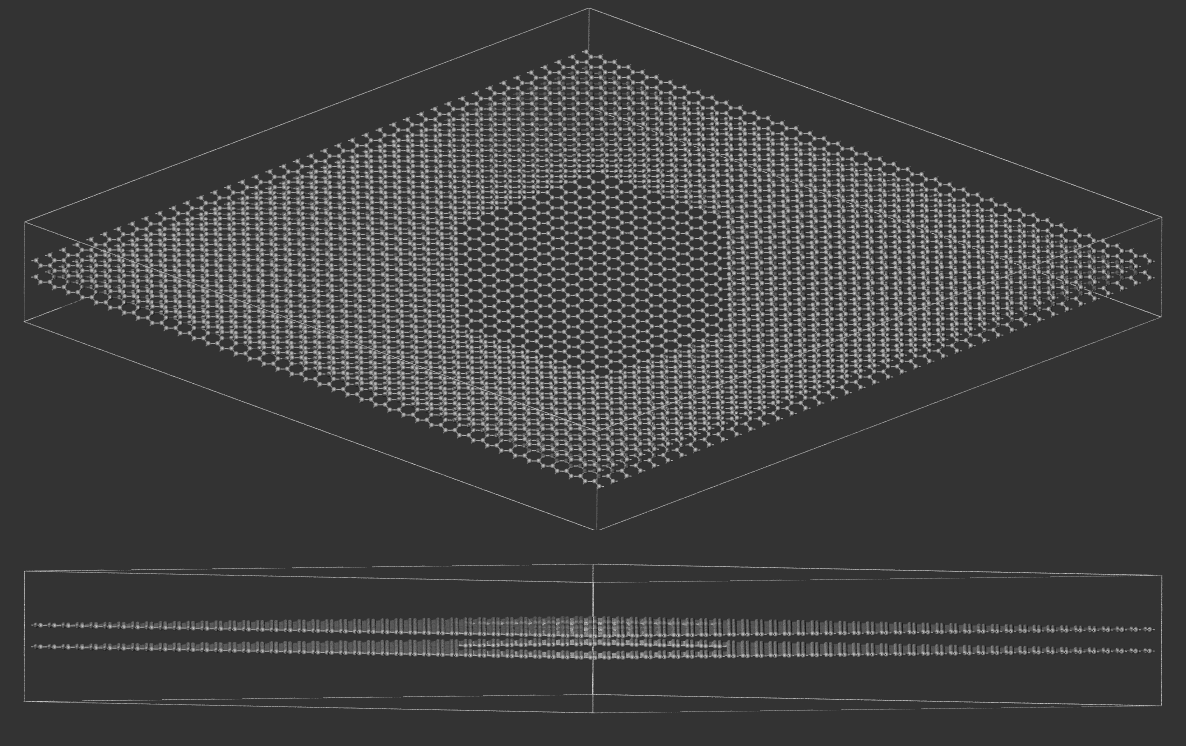
\includegraphics[width=\columnwidth]{Figures/DoubleMembrane.png}
  \end{figure}
 \end{columns}
\end{frame}

\subsection{Visualising Modes}

\begin{frame}
 \frametitle{Visualising Modes}
 \begin{columns}[T]
  \column{0.75\textwidth}
  \animategraphics[width=\columnwidth]{30}{VNL/Clamped/frame}{0}{29}
  \begin{center}
   Clamped system
  \end{center}
  \column{0.75\textwidth}
  \animategraphics[width=\columnwidth]{30}{VNL/Substrate/frame}{0}{29}
  \begin{center}
   Supported system
  \end{center}
 \end{columns}
\end{frame}

\subsection{Extracting Modes}

\begin{frame}
 \frametitle{Extracting Modes}
 \begin{listing}[H]
  \inputminted[python3=true,bgcolor=Black,linenos=true,firstline=66,lastline=71,breaklines=true,breakautoindent=true]{python}{VNL/PythonScripts/Scripts/2DdataExtract.py}
 \end{listing}
 \begin{itemize}[<+->]
  \pause
  \item ATKPython
  \item Matplotlib \& Pyplot
 \end{itemize}
\end{frame}

\section{Our Findings}

\subsection{Frequencies vs size}

\begin{frame}
 \frametitle{Frequencies vs size}
 \begin{center}
  Clamped System
 \end{center}
 \begin{columns}[T]
  \column{0.8\textwidth}
  \includegraphics[width=\columnwidth]{Figures/FrequencyModeProjectionsNoZoom.eps}
  \column{0.8\textwidth}
  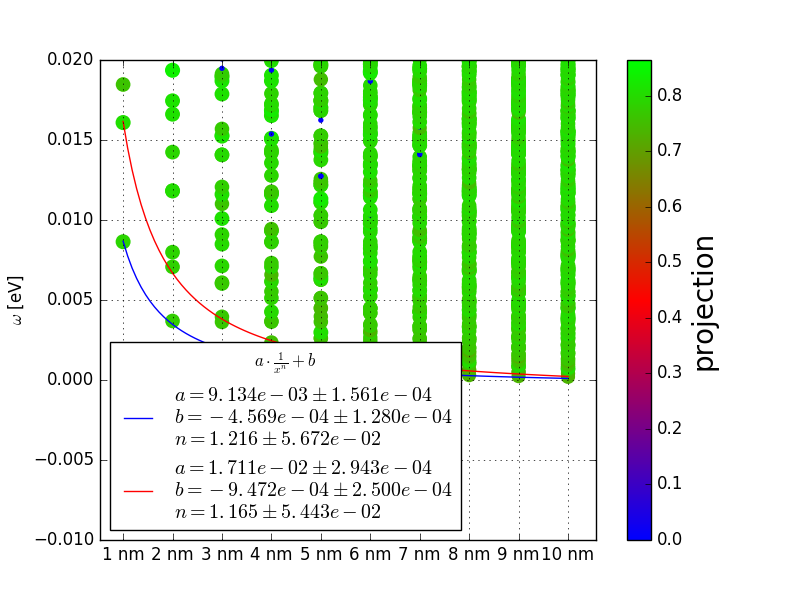
\includegraphics[width=\columnwidth]{Figures/FrequencyModeProjectionsZoomFit.eps}
 \end{columns}
\end{frame}

\begin{frame}
 \frametitle{Frequencies vs size}
 \begin{center}
  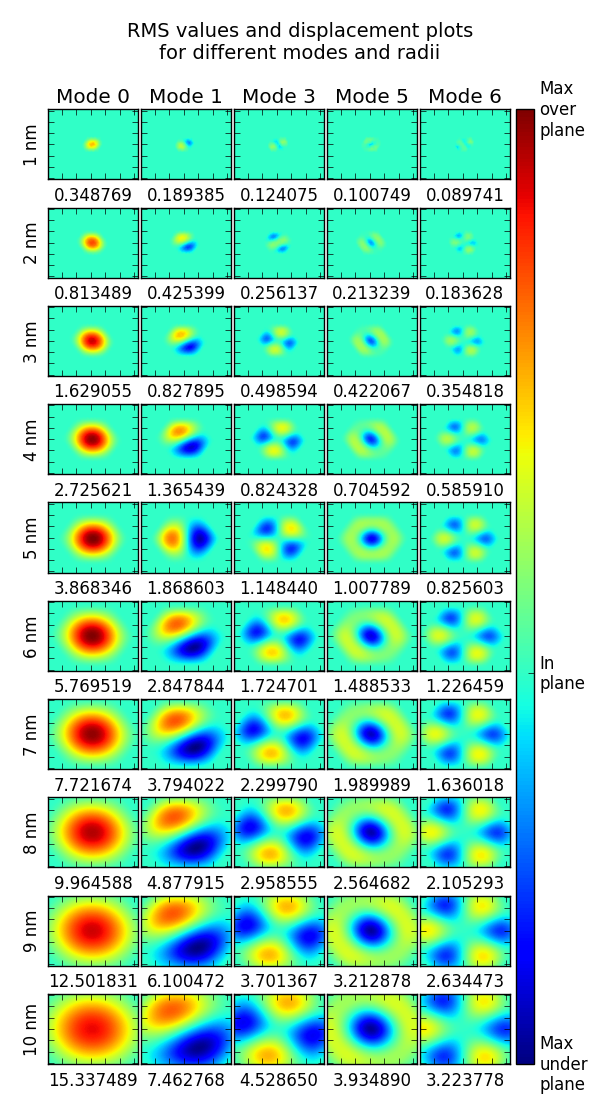
\includegraphics[width=0.4\textwidth]{Figures/2DRMSClamped.eps}
 \end{center}
\end{frame}

\subsection{Clamped vs Supported Systems}

\begin{frame}
 \frametitle{Clamped vs Supported Systems}
 \begin{columns}[T]
  \column{0.7\textwidth}
  \includegraphics[width=\columnwidth]{Figures/FrequencyModeProjectionsZetaNoZoom.eps}
  \column{0.7\textwidth}
  \includegraphics[width=\columnwidth]{Figures/FrequencyModeProjectionsZeta.eps}
 \end{columns}
 \begin{equation}
  V_{ij}(r) = 4 \epsilon_{ij} \left[ \left( \frac{\sigma_{ij}}{r} \right) ^{12} - \left( \frac{\sigma_{ij}}{r} \right) ^6 \right] \nonumber
 \end{equation}
\end{frame}

\begin{frame}
 \frametitle{Clamped vs Supported Systems}
 \begin{center}
  \includegraphics[width=0.9\textwidth]{Figures/2DRMS.eps}
 \end{center}
\end{frame}

\section{Conclusion}

\begin{frame}
 \frametitle{Conclusion}
 \begin{columns}[T]
  \column{0.7\textwidth}
  \begin{itemize}
   \item<2-> Simulation enviroment works
   \item<3-> Geometric behavior similar to Vibrational Nanodrums
   \item<4-> Vibrational modes are theoretically scaleable to nanoscale
   \item<5-> Next step: Molecular Dynamics, Hole Coupling and Experimental testing
  \end{itemize}
  \column{0.7\textwidth}<5->
  \begin{center}
   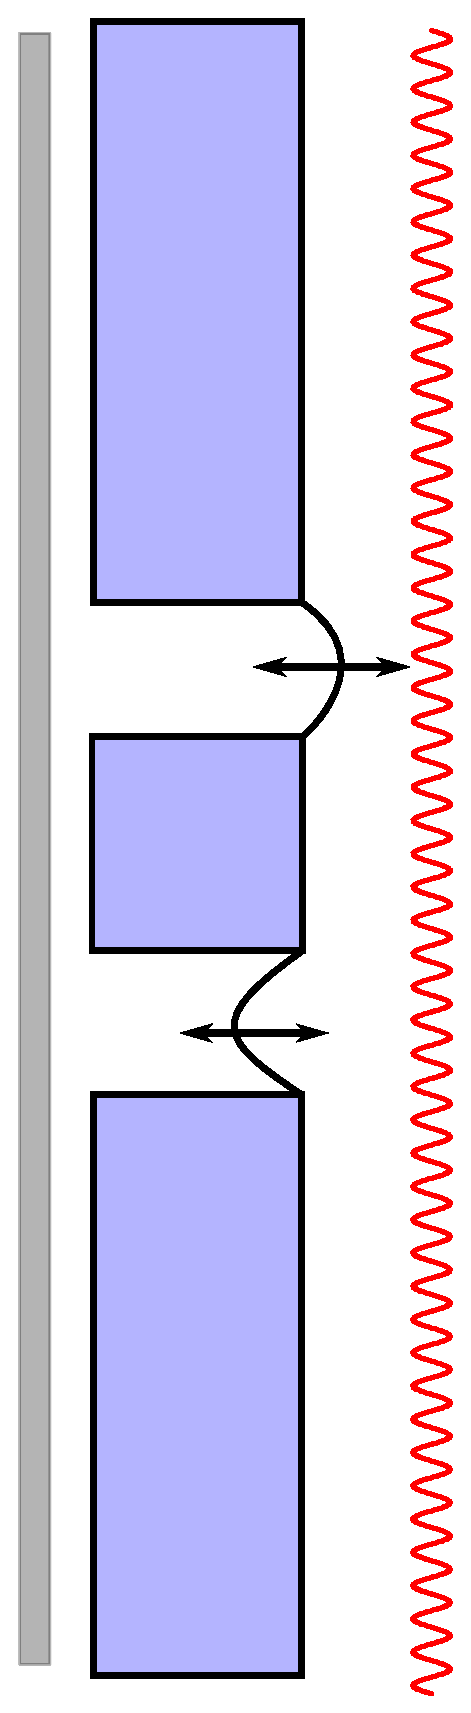
\includegraphics[height=0.6\textheight]{Figures/Fuck_dig_christoffer.eps}
  \end{center}
 \end{columns}
\end{frame}

\section*{Questions}
\title{Questions}
\subtitle{}
\begin{frame}
 \titlepage
\end{frame}

\end{document}
